\subsection{Формула тонкой линзы}

\begin{wrapfigure}[9]{c}{0.6\tw}
    \centering
    \vspace{-1pc}
    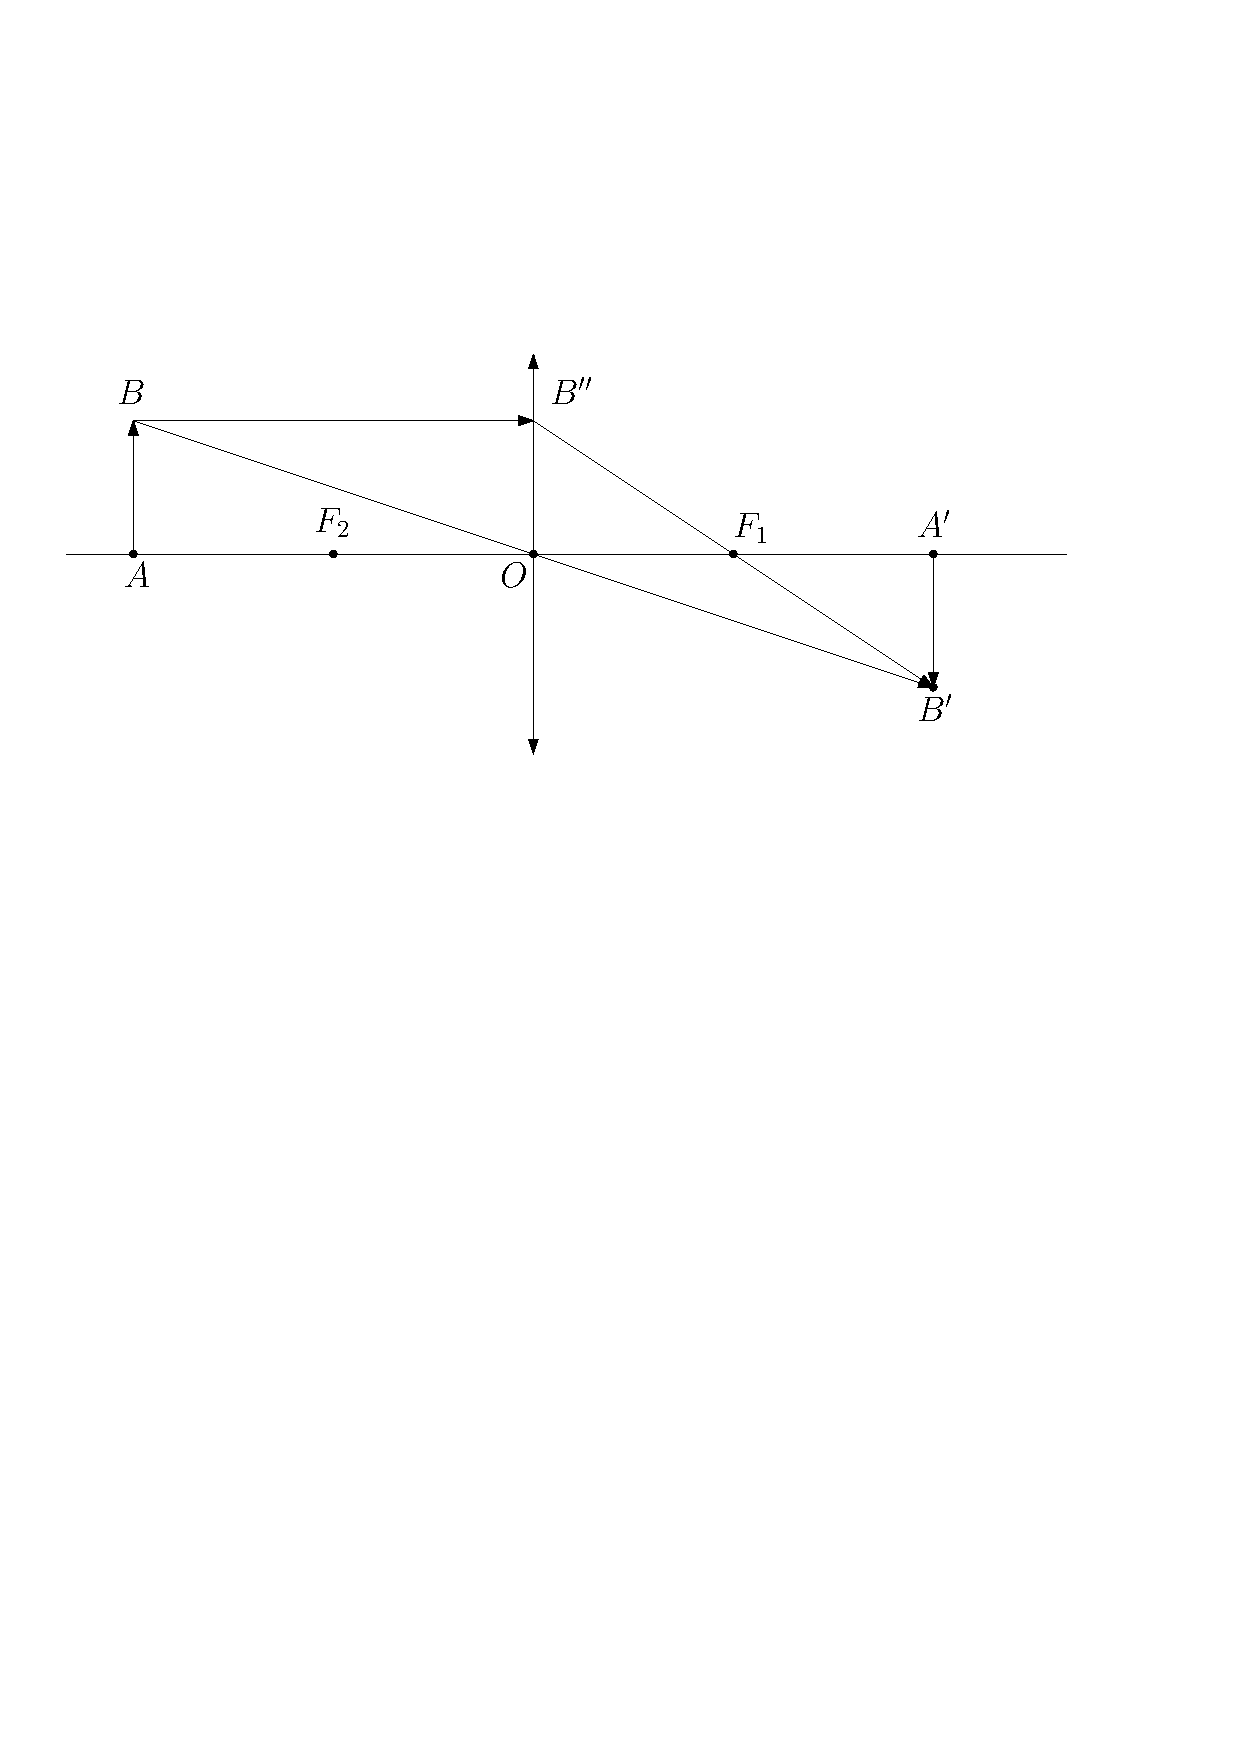
\includegraphics[width=.6\tw]{thin-lense}
    \caption{Схема лучей в тонкой линзе}
    \label{fig:thin-lens}
\end{wrapfigure}

Выведем формулу для связи расстояния от объекта до линзы, расстояния до изображения и фокусным расстоянием линзы.
Введем обозначения: $F = OF_1 = OF_2$~--- фокусное расстояние линзы, $d = OA = BB^{\prime \prime}$~--- расстояние до объекта, $f = OA^\prime$~--- расстоние до изображения.
\begin{equation}
    \Delta ABO \sim \Delta A^\prime B^\prime O \Longrightarrow \frac{d}{f} = \frac{OB}{OB^\prime} = \frac{AB}{A^\prime B^\prime}
\end{equation}
\begin{equation}
    \Delta OB^{\prime \prime} F_1 \sim \Delta A^\prime B^\prime F_1 \Longrightarrow \frac{f - F}{F} = \frac{F_1 B^\prime}{OF_1} = \frac{A^\prime B^\prime}{OB^{\prime \prime}} = \frac{A^\prime B^\prime}{AB}
\end{equation}
\begin{equation}
    \frac{f}{d} = \frac{f - F}{F} \Longrightarrow \frac{1}{d} = \frac{1}{F} - \frac{1}{f} \Longrightarrow \frac{1}{F} = \frac{1}{f} + \frac{1}{d}
\end{equation}
Полученная формула называется формулой тонкой линзой.

